% The class loads biblatex with backend=biber. This starter's compile
% pipeline runs the classic bibtex/(pdf|xe|lua)latex cycle (no biber pass), so
% the backend is switched to bibtex here, before the class loads biblatex —
% biblatex silently accepts a plain .bib file either way.
\PassOptionsToPackage{backend=bibtex}{biblatex}
\documentclass[9pt,a4paper,twocolumn,twoside]{rho-class/rho}
\usepackage[english]{babel}

%----------------------------------------------------------
% Math macros
%----------------------------------------------------------
\usepackage{amsmath,amssymb,amsfonts}%
\usepackage{tensor}
\usepackage{upgreek}
\usepackage{sansmath}
\usepackage{xspace}
\usepackage{array}
\usepackage{mathtools}
\newcommand{\bm}[1]{\text{\boldmath{$#1$}}}

\graphicspath{{../results/}, {../figures/}}

%----------------------------------------------------------
% Title
%----------------------------------------------------------

\doctype{Lab Report}
\title{Experiment 1: Uniaxial Tensile Test of Polycarbonate Sample}

%----------------------------------------------------------
% Authors, affiliations and dates
%----------------------------------------------------------

\author[a,1]{Vilmer Dahlberg}

\affil[a]{Department of Construction Sciences, Lund University}

\dates{Manuscript compiled \today}

\docinfo{This article was prepared with the rho-class LaTeX template and compiled with pdfLaTeX.}

%----------------------------------------------------------
% Abstract and keywords
%----------------------------------------------------------

\begin{abstract}
	Replace this abstract with a concise, self-contained summary of the
	paper: the problem addressed, the method used, and the main result.
	Two to four sentences is typical for a research article.
\end{abstract}

\begin{document}
	
	\maketitle
	
	\section{Introduction}
	Polycarbonate is a type of thermoplastic polymer which, due to its malleability, high strength and toughness, can be found in many modern engineering applications \cite{wikipedia_polycarbonate}. To gain further insight into the material properties of polycarbonate, we perform in this experiment a uniaxial tensile test. The polycarbonate specimen, shown in Figure \ref{fig:method:setup}a consists of a thin rectangular brick with two vertically centered circular notches. The specimen is mounted in a tensile testing rig, which consists of a) a motor which pulls the specimen at a constant rate of displacement (it est displacement controlled loading) and b) a load cell which measures the force required to pull the specimen apart. The data is recorded in a LABVIEW \cite{national_instruments_labview_2017} program.
	
	To measure the force we use a load cell, which in this experiment consists, of a metal body fitted with a strain gauge. As the load cell deforms due to the external load, the strain gauge deforms, causing a change in electrical resistance. This small difference is measured as a change in voltage and converted into a strain. The stress can then be computed under the assumption of elastic response, which finally gives the force \cite{wikipedia_load_cell}.
	
	Given a cross-section of a continuum body at some spatial point $\bm{x}$ with area $A$ and normal $\bm{n}$ we define the stress vector $\bm{s}$ at that point as
	$$
		\bm{s} = \bm{\sigma}\bm{n} = \lim_{\Delta \bm{A} \rightarrow 0} \frac{\Delta \bm{P}}{\Delta A}
	$$
	where $\Delta \bm{P}$ the measured traction. Unfortunately, it is in practice impossible to measure the stress directly, for many reasons. Firstly, it's a destructive process, meaning it can realistically only be done once before the specimen is destroyed. Secondly, it is impossible to make cross sections with infinitesimally small areas and thirdly any such cross-sections would immediately be out of static equilibrium. Instead we rely on proxies, such as strain, or simplified geometries.

	
	For instance, consider a cylindrical rod $\mathcal{R}$ with initial length and cross-sectional area $l_0$ and $A_0$ consisting of a homogeneous material. When subjected to a force $P$ along its axial direction the rod will have the new length and cross-sectional areas $l$ and $A$. The (small strain) stretch along its axial direction is given by 
	$$
		\epsilon_E = \frac{l-l_0}{l_0} \implies \frac{V}{V_0} = \frac{lA}{l_0A_0} = \left(\epsilon_E + 1\right)\frac{A}{A_0}
	$$
	Furthermore, mechanical equilibrium requires the stress to be equal for any axial-orthogonal cross-section. We are then able to define the \textit{engineering} and \textit{true} stress as
	\begin{align*}
		  \sigma_E 	& = \frac{P}{A_0} %
		& \sigma_T	& = \frac{P}{A}
	\end{align*}
	which are related via 
	\begin{equation*}
		\sigma_T = \sigma_E\frac{V}{V_0}\left(\epsilon_E + 1\right)
	\end{equation*}
	
	\section{Method}
	Firstly the specimen's dimensions are measured using a caliper. The recorded lengths are shown in Table \ref{tab:method:polycarbonate dimensions.}.
	
	\begin{table}
		\caption{Recorded dimensions of polycarbonate sample, in millimeters $[mm]$.}
		\centering
		\begin{tabular}{c|c|c|c|c}
			$L_1$ 	& $L_2$	& $w_1$	& $w_2$ & $t$ 	\\
			\hline
			80.6	& 10.0	& 25.5	& 9.7 	& 3.1 	\\
		\end{tabular}
		\label{tab:method:polycarbonate dimensions.}
	\end{table}
	
	The sample is then loaded into the machine, as shown in Figure \ref{fig:method:setup}b. To ensure that no adversarial torsional forces are applied to the sample during loading, the holding grips are held in place while they are tightened. Once the specimen is loaded into the rig, its height is measured.
	
	The tensile loading machine is set to displacement controlled loading at a constant rate of $2\,\text{mm}/60\text{s}$. The machine and data acquisition are then simultaneously started. The tensile testing machine is then allowed to run until the sample fails, see Figure \ref{fig:method:setup}c, at which point the machine and recording software are stopped simultaneously.

	\begin{figure}
		\centering
		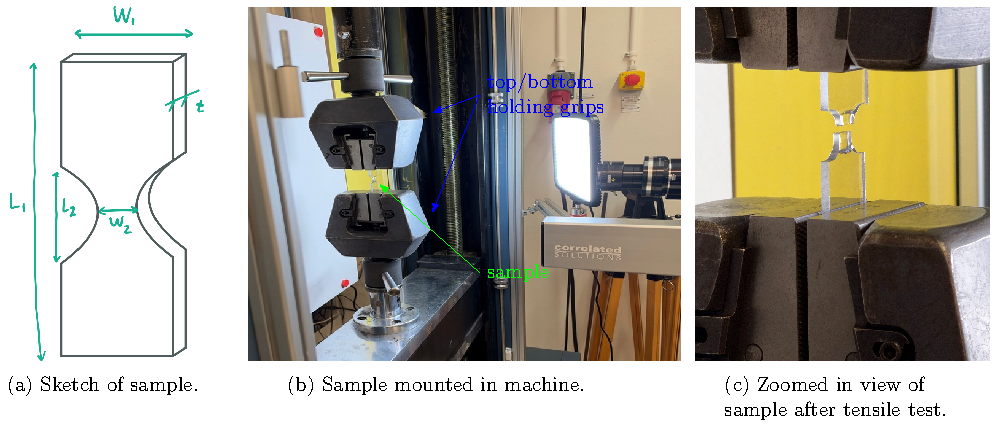
\includegraphics[width=0.5\textwidth]{figure_mosiac.pdf}
		\caption{Mosaic of experimental set-up}
		\label{fig:method:setup}
	\end{figure}
	
	\section{Results}
	The acquired force-displacement data is shown in Figure \ref{fig:force_displacement}.
	\begin{figure}[t]
		\centering
		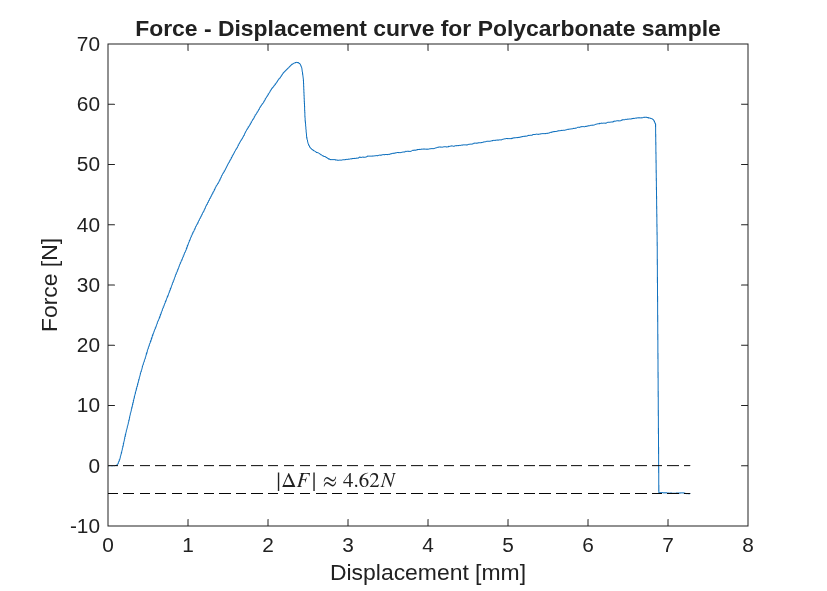
\includegraphics[width=10cm]{force_displacement.png}
		\caption{Plot of the force-time data gathered during the tensile test. The force-displacement graph can be inferred from the displacement rate by scalar multiplication.}
		\label{fig:force_displacement}
	\end{figure}
	
	
	\section{Discussion}
	Some points i would like to discuss.
	\begin{itemize}
		\item[] You'd expect the curve to be linear initially, but it does not look like it. 
		\item[] Directly after the maximum load there is a decrease in force, this happens because we are using a displacement controlled loading. But maybe if we were to use a path following scheme we could trace the snap-back.
		\item[] After the drop there is a subsequent small increase in load, after failure finally occurs at circa 50N.
		\item[] What i personally find interesting is that we see no hysteresis, which is maybe what you would expect from polycarbonate.
		\item[] We also note (and maybe should begin with) the fact that we are looking at force-displacement data, and not a stress/strain relationship. Therefore it is hard to do any comparison between the results and any material model, which requires local data. This could be improved somewhat by doing a DIC, but the stress information is either way unknown.
		\item[] Discrepancy in "zero" force between start and end of test
		\item[] Poisson effect
	\end{itemize}
	
	\section{Conclusions}
	
	
	\printbibliography
	
\end{document}
